\documentclass[tikz,border=10pt]{standalone}
\usepackage{tikz}
\usetikzlibrary{shapes,arrows,positioning}
\usepackage{amsmath}

\definecolor{fepblue}{RGB}{41,128,185}
\definecolor{crrgreen}{RGB}{39,174,96}
\definecolor{goalred}{RGB}{192,57,43}
\definecolor{matchpurple}{RGB}{142,68,173}

\begin{document}
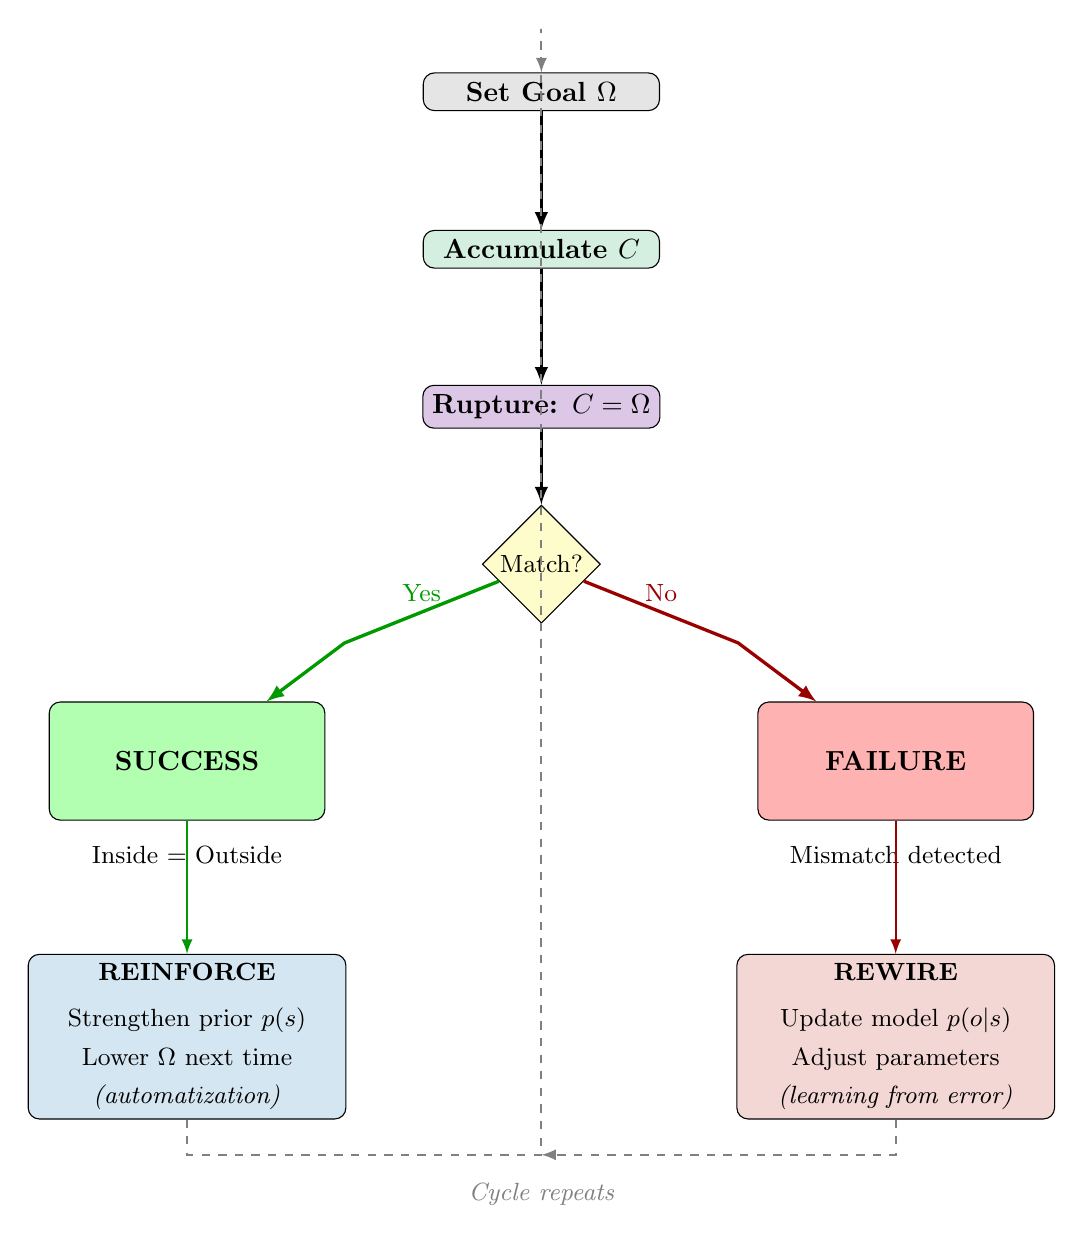
\begin{tikzpicture}[scale=1]
% Main flow
\node[draw, rounded corners, fill=gray!20, minimum width=30mm, font=\bfseries] (goal) at (0,5) {Set Goal $\Omega$};
\node[draw, rounded corners, fill=crrgreen!20, minimum width=30mm, font=\bfseries] (accum) at (0,3) {Accumulate $C$};
\node[draw, rounded corners, fill=matchpurple!30, minimum width=30mm, font=\bfseries] (rupture) at (0,1) {Rupture: $C = \Omega$};

\draw[-latex, very thick] (goal) -- (accum);
\draw[-latex, very thick] (accum) -- (rupture);

% Branch point
\node[draw, diamond, fill=yellow!20, minimum width=15mm, minimum height=15mm] (branch) at (0,-1) {};
\node[font=\small] at (0,-1) {Match?};

\draw[-latex, very thick] (rupture) -- (branch);

% Success branch
\node[draw, rounded corners, fill=green!30, minimum width=35mm, minimum height=15mm, font=\bfseries] (success) at (-4.5,-3.5) {SUCCESS};
\node[below=2mm of success, font=\small] {Inside = Outside};

% Failure branch
\node[draw, rounded corners, fill=red!30, minimum width=35mm, minimum height=15mm, font=\bfseries] (fail) at (4.5,-3.5) {FAILURE};
\node[below=2mm of fail, font=\small] {Mismatch detected};

\draw[-latex, very thick, green!60!black] (branch) -- node[above, font=\small] {Yes} (-2.5,-2) -- (success);
\draw[-latex, very thick, red!60!black] (branch) -- node[above, font=\small] {No} (2.5,-2) -- (fail);

% Outcomes
\node[draw, rounded corners, fill=fepblue!20, minimum width=40mm, text width=38mm, align=center, font=\small] (reinforce) at (-4.5,-7) {
\textbf{REINFORCE}\\[2mm]
Strengthen prior $p(s)$\\[1mm]
Lower $\Omega$ next time\\[1mm]
\emph{(automatization)}
};

\node[draw, rounded corners, fill=goalred!20, minimum width=40mm, text width=38mm, align=center, font=\small] (rewire) at (4.5,-7) {
\textbf{REWIRE}\\[2mm]
Update model $p(o|s)$\\[1mm]
Adjust parameters\\[1mm]
\emph{(learning from error)}
};

\draw[-latex, thick, green!60!black] (success) -- (reinforce);
\draw[-latex, thick, red!60!black] (fail) -- (rewire);

% Return arrows
\draw[-latex, thick, dashed, gray] (reinforce.south) -- (-4.5,-8.5) -- (0,-8.5) -- (0,5.8) -- (goal.north);
\draw[-latex, thick, dashed, gray] (rewire.south) -- (4.5,-8.5) -- (0,-8.5);

\node[gray, font=\small\itshape] at (0,-9) {Cycle repeats};
\end{tikzpicture}
\end{document}
